\chapter{Computational Drug Discovery}

Databases
  PDB \citep{105}

Reviews
  anticancer drug development \citep{254}

Early drug discovery
  Generalized Centroid Estimators in Bioinformatics \citep{272}

Drug discovery via merely biological and chemical means are both cost-inefficient and time-inefficient. A computational framework for fast and accurate drug discovery is thus highly appreciated. The thesis concentrates on building computer models to simulate the three early stages of modern drug discovery process, namely hit identification, lead identification and lead optimization. From the computational perspective, they typically involve binding site identification, structure-based virtual screening, computational synthesis of potent ligands, drug properties prediction, interactive visualization, and so on. The thesis addresses structure-based virtual screening and computational synthesis of potent ligands.

Meanwhile, general-purpose computing on Graphics Processing Unit (GPU) is gaining more and more popularity in computationally intensive fields such as drug discovery.

\section{Structure-Based Virtual Screening}

As the X-ray crystallography and Nuclear Magnetic Resonance (NMR) technologies evolve, more and more 3D structures of biological macromolecules at atomic level have been revealed and deposited into the world's largest repository PDB (Protein Data Bank) \citep{540,539,537,105,538}. This rapid evolution catalyzes the development of various algorithms and tools for structure-based drug discovery via protein-ligand docking.

Protein-ligand docking is a method which predicts the preferred conformation (i.e. position and orientation) of a small ligand when bound to a macro protein to form a stable complex (Figure \ref{fig:Docking}, reprinted from Wikipedia). It also predicts the binding affinity in terms of free energy, which is basically the overall effect of various chemical forces involved, such as van der Waals force, electrostatic force, hydrogen bonding, hydrophobic interactions, Pi-Pi interactions, and the like. Free energy measures the degree of freedom of the ligand to ``escape'' from the protein, so the lower the free energy, the higher the binding affinity. Very often, the target protein is a viral enzyme of interest, and the small organic ligands that are predicted to inhibit the viral enzyme are what we want to discover.

\begin{figure}[t]
\centering
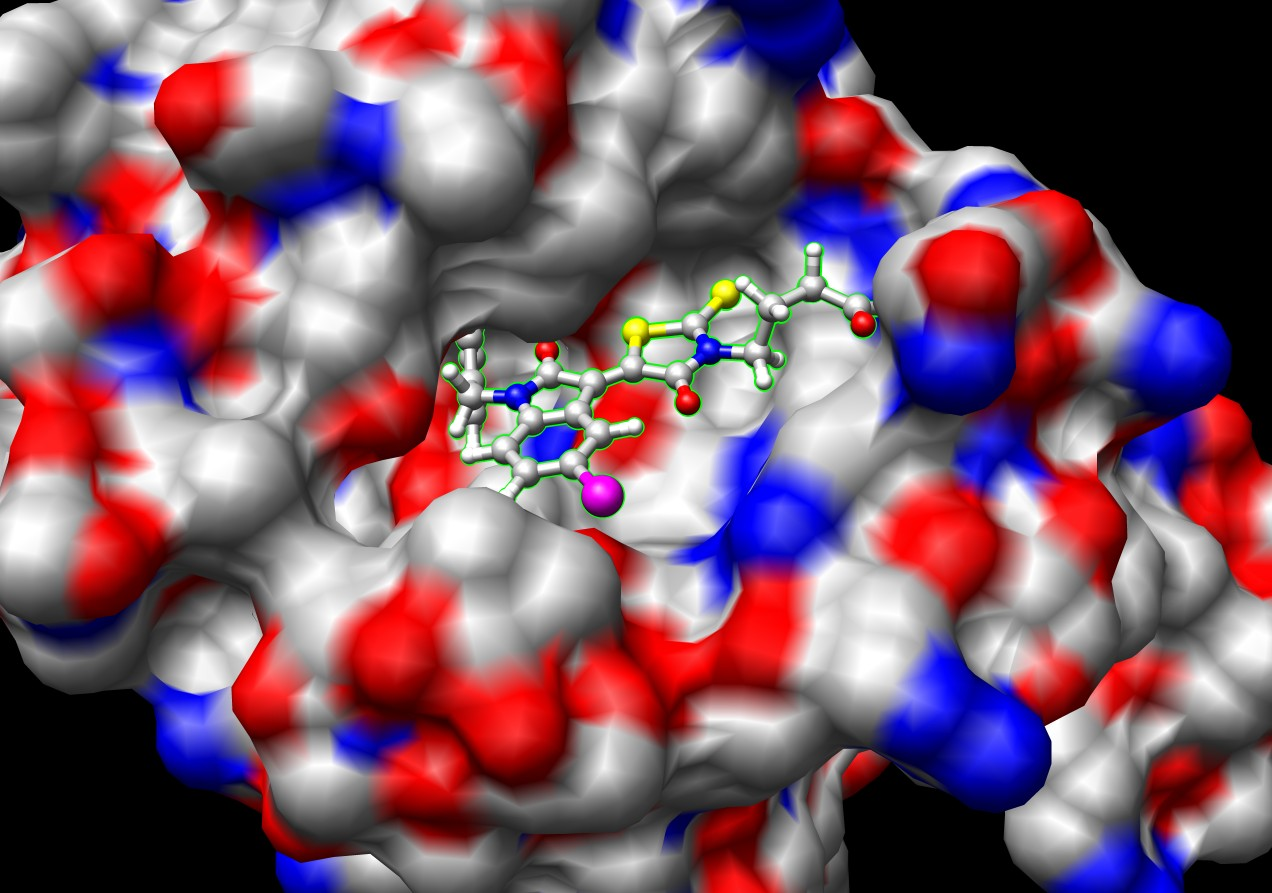
\includegraphics[width=\textwidth]{Background/Docking.jpg}
\caption{A ligand docked against a protein. Figure reprinted from Wikipedia.}
\label{fig:Docking}
\end{figure}

Docking programs typically consist of two basic components, a scoring function to predict the binding affinity, and an algorithm to explore the conformational space of the ligand and the protein \citep{493}. So far, dozens of scoring functions \citep{579,566,570,775,575,576,578,580,581,774} and dozens of algorithms \citep{595,564,594,602,603,604,605,606,607,781,614,615,617} have been developed. Some methods have been comprehensively evaluated and compared \citep{637,771,556}.

Among the many docking programs, AutoDock Vina \citep{595} (hereafter Vina for short) is a competitive one. It's free and open source. It runs faster than its predecessor AutoDock4 \citep{596} by an order of magnitude \citep{556}. Released in 2010, Vina has been cited by 117 other publications and adopted by many researchers \citep{609}. Indeed, it is intensively used in our research projects too.

Virtual screening is simply a massive version of docking (Figure \ref{fig:VirtualScreening} \citep{470}). It docks a database of drug-like ligands to a viral protein of interest, ranks them according to their predicted binding affinity, and shortlists the best ones for further investigation. Statistical frameworks and assessments have been established for evaluation and result selection \citep{489,491,769,583,582}. In reality, docking and virtual screening have successful applications for drug discovery \citep{495,498,751,503,752,757,506,738,761,763,766,736}.

\begin{figure}
\centering
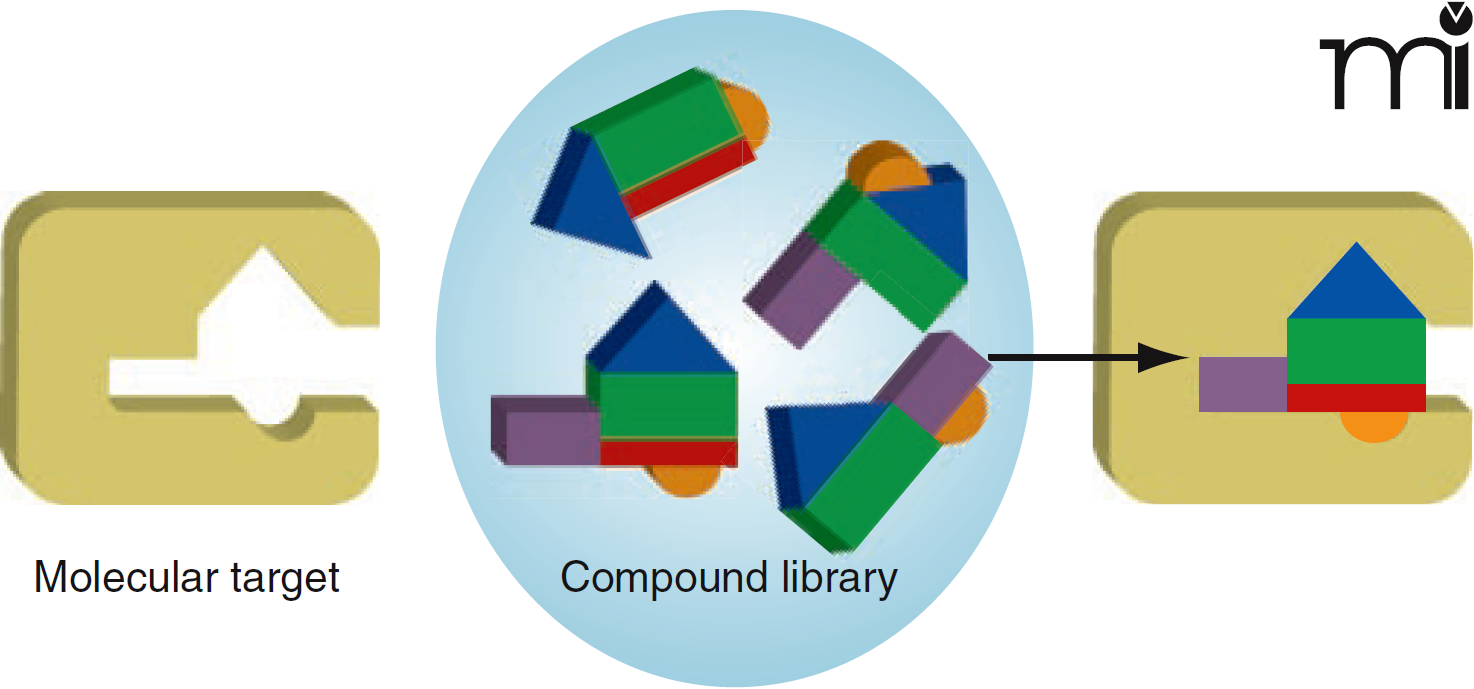
\includegraphics[width=\textwidth]{Background/VirtualScreening.png}
\caption{Virtual screening to identify compounds that bind to the target. Figure reprinted from \citep{470}.}
\label{fig:VirtualScreening}
\end{figure}

There are quite a lot data sources and databases for virtual screening, such as PDB \citep{540,539,537,105,538}, ZINC \citep{532}, PDBbind \citep{529,530}, and PubChem \citep{526}. In addition to raw data, there are library analysis \citep{521}, benchmark datasets \citep{534,533,535,536}, and data mainipulation tools \citep{542}. Some tools exploit massive parallelism in the form of either cluster computing or cloud computing \citep{557,773,560,782}.

\section{Computational Synthesis of Potent Ligands}

Virtual screening tries to discover promising ligands out of a database. Apparently the diversity of its outcome is limited to the diversity of the database. In other words, if the database contains no promising ligands at all, virtual screening will not succeed.

In contrast, computational synthesis produces novel molecular structures with desired pharmacological properties from scratch. Figure \ref{fig:ComputationalSynthesis} shows the relationship between synthesis and docking. Figure \ref{fig:LigandDesign} \citep{363} illustrates three kinds of strategies for ligand design. A number of compounds that evolved from fragments have entered the clinic, and the approach is increasingly accepted as an additional route to identifying new hits in inhibitor design \citep{363,470}.

\begin{figure}
\centering
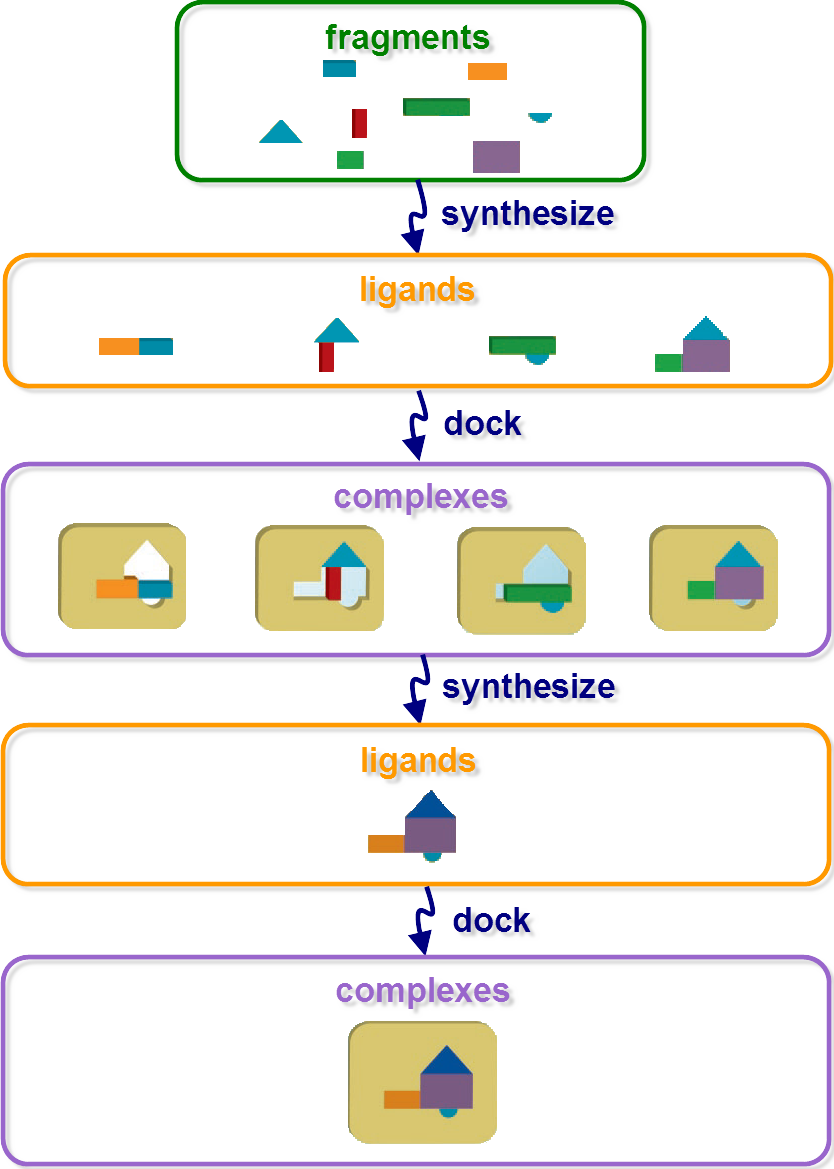
\includegraphics[width=\textwidth]{igrow/ComputationalSynthesis.png}
\caption{Synthesizing ligands from fragments followed by docking.}
\label{fig:ComputationalSynthesis}
\end{figure}

\begin{figure}[t]
\centering
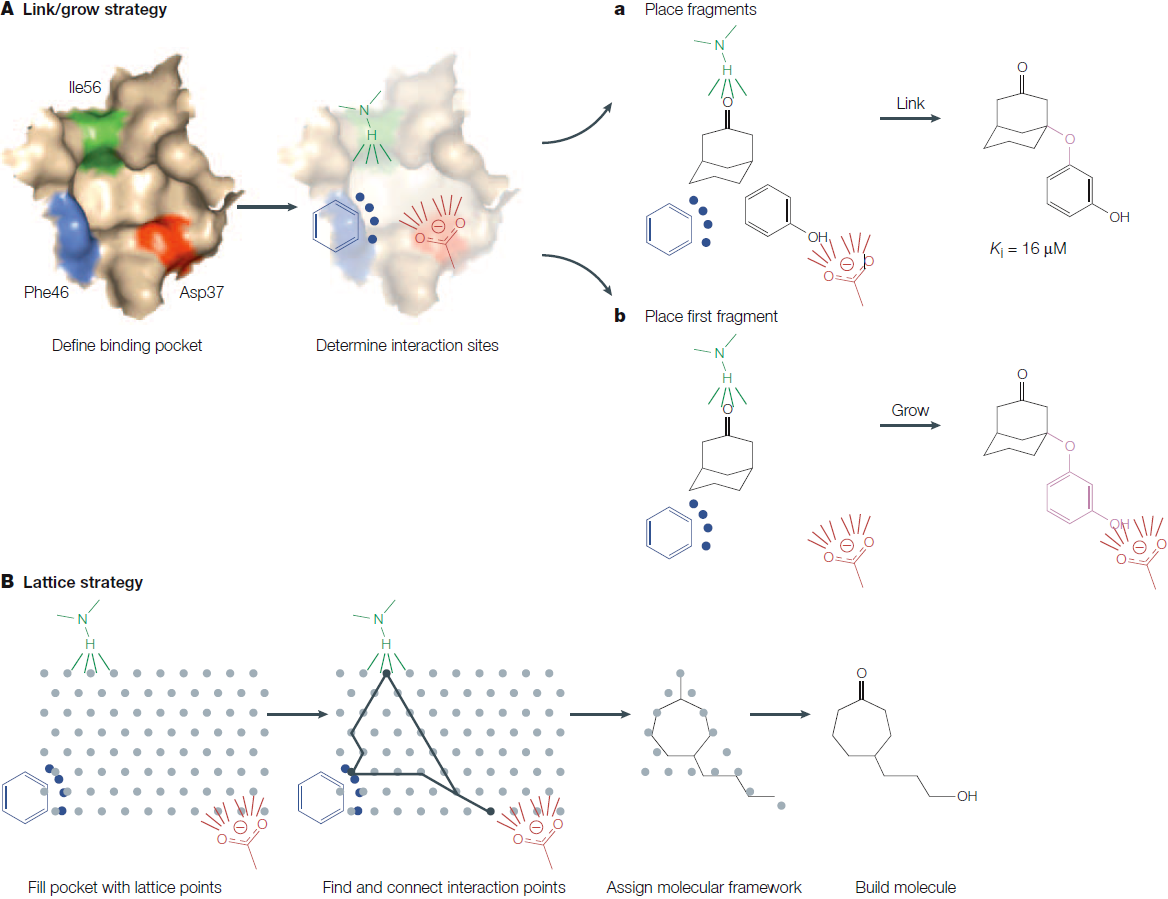
\includegraphics[width=\textwidth]{igrow/LigandDesign.png}
\caption{Ligand design strategies. Figure reprinted from \citep{363}.}
\label{fig:LigandDesign}
\end{figure}

A computational synthesis program is confronted with a virtually infinite search space. The number of chemically feasible, drug-like molecules has been estimated to be in the order of 10\textsuperscript{60} to 10\textsuperscript{100} \citep{363}, from which the most promising candidates have to be selected and synthesized. Rather than the systematic construction and evaluation of each individual compound, computational synthesis programs rely on the principle of local optimization, which does not necessarily lead to the globally optimal solution. In fact, most software implementations \citep{466,749} are non-deterministic, and rely on some kind of stochastic structure optimization.

Among the many ligand synthesis programs, AutoGrow \citep{466} is a representative one which implements genetic algorithm to create a population of ligands. It is the only ligand synthesis program that uses Vina \citep{595} as external docking engine for the selection operator. It is free and open source. However, it requires messy configurations and its performance is hardly considered to be amazing. Hence its userbase is rather limited and has been cited by merely 8 other publications since it was born in 2009. It is used as a baseline tool in our research projects.

\section{General-Purpose Computing on GPU}

Nowadays the explosively growing size of biological data together with the high complexity of bioinformatics algorithms demand more powerful parallel machines. However, such high performance computers are only available in bioinformatics centers due to their sky-high price. Hence, cloud and heterogeneous computing are emerging as solutions for tackling large-scale and high dimensional data sets \citep{269,267,268}. In particular, the modern GPU has evolved from a fixed-function graphics pipeline to a programmable parallel processor with extremely high computational throughput and tremendous memory bandwidth at an affordable price, enabling researchers to study bioinformatics in more details within less time.

There are quite a few successful GPU applications in drug discovery, including binding site mapping \citep{722}, molecular docking \citep{723,652,779}, chemical similarity calculation \citep{726}, and compound selection \citep{750}.

GPU applications in bioinformatics
  sequence alignment \citep{123,1064}
  protein database search \citep{189}

In November 2006, NVIDIA announced Compute United Device Architecture (CUDA). In December 2008, the Khronos Group released the first specification of Open Computing Language (OpenCL). Both techniques greatly reduce the GPU programming complexity and saves programmers from learning traditional graphics pipelines. More and more computationally intensive problems, ranging from computational biology to computational chemistry, have been successfully ported to the GPU and gained speedups from 10x to 1000x compared to single threaded CPU counterparts.

NVIDIA’s latest GPU architecture, codenamed “Kepler,” create an extremely power-efficient GPU
The first GPU based on our new Kepler architecture, codenamed “GK104,” every internal unit was designed for the best perf/watt possible
Kepler GPUs are composed of different configurations of Graphics Processing Clusters (GPCs), Streaming Multiprocessors (SMs), and memory controllers. The GeForce GTX 680 GPU consists of four GPCs, eight next-generation Streaming Multiprocessors (SMX), and four memory controllers. In GeForce GTX 680, each GPC has a dedicated raster engine and two SMX units. With a total of eight SMX units, the GeForce GTX 680 implementation has 1536 CUDA Cores. The SM is the heart of NVIDIA’s unified GPU architecture. Most of the key hardware units for graphics processing reside in the SM. Special Function Units (SFUs) handle transcendental and graphics interpolation instructions. To feed the execution resources of SMX, each unit contains four warp schedulers, and each warp scheduler is capable of dispatching two instructions per warp every clock.

Each of the Kepler GK110 SMX units feature 192 single‐precision CUDA cores, and each core has fully pipelined floating‐point and integer arithmetic logic units. Kepler retains the full IEEE 754‐2008 compliant single‐ and double‐precision arithmetic introduced in Fermi, including the fused multiply‐add (FMA) operation.

The SMX schedules threads in groups of 32 parallel threads called warps. Each SMX features four warp schedulers and eight instruction dispatch units, allowing four warps to be issued and executed concurrently. Kepler’s quad warp scheduler selects four warps, and two independent instructions per warp can be dispatched each cycle.

special function units (SFUs) for fast approximate transcendental operations

Figure \ref{GPU:GeForceGTX680BlockDiagram}
Figure \ref{GPU:GeForceGTX680SMX}

\begin{figure}
\centering
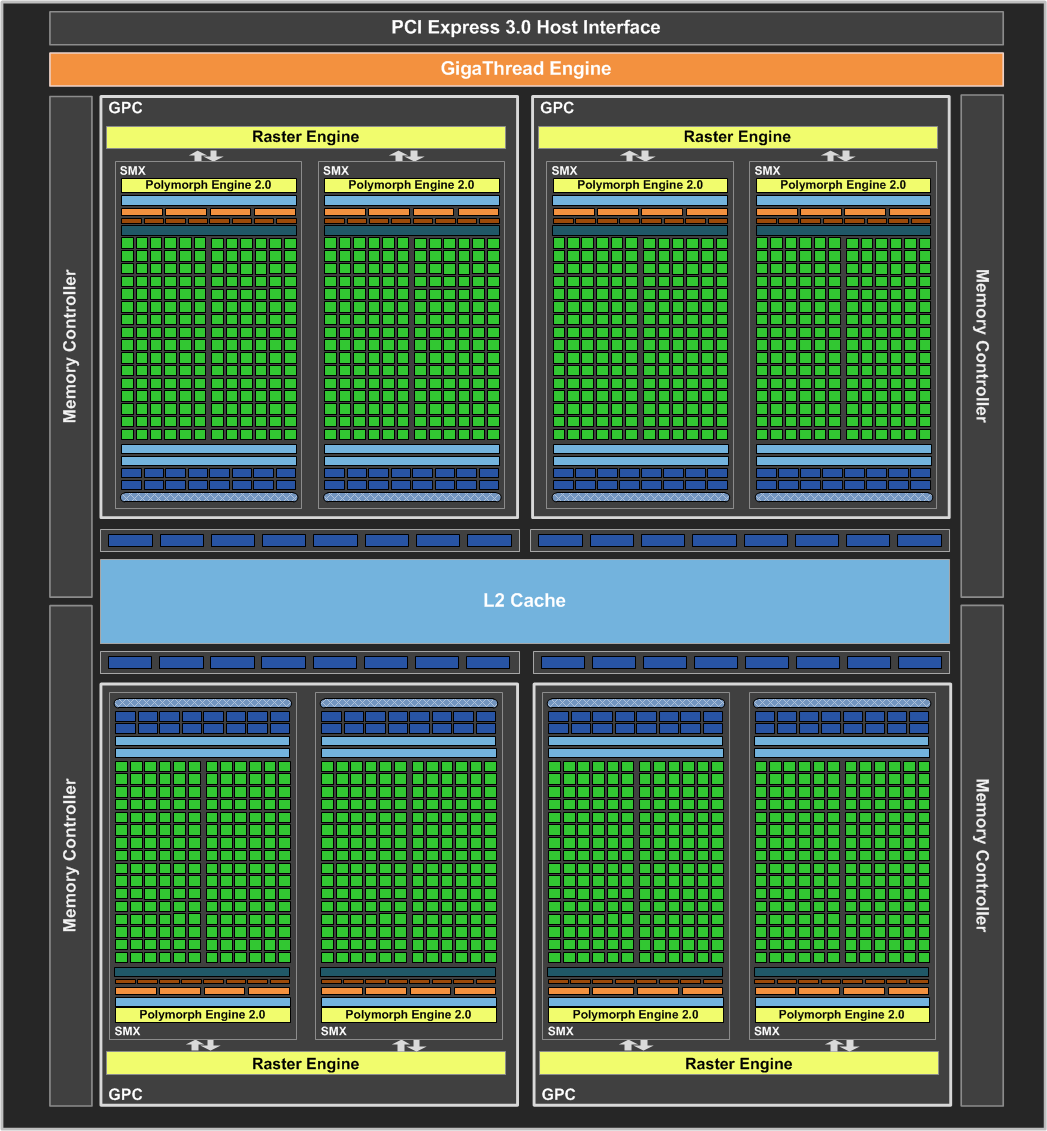
\includegraphics[width=\textwidth]{GPU/GeForceGTX680BlockDiagram.png}
\caption{NVIDIA GeForce GTX680 Block Diagram. Source: NVIDIA.}
\label{GPU:GeForceGTX680BlockDiagram}
\end{figure}

\begin{figure}
\centering
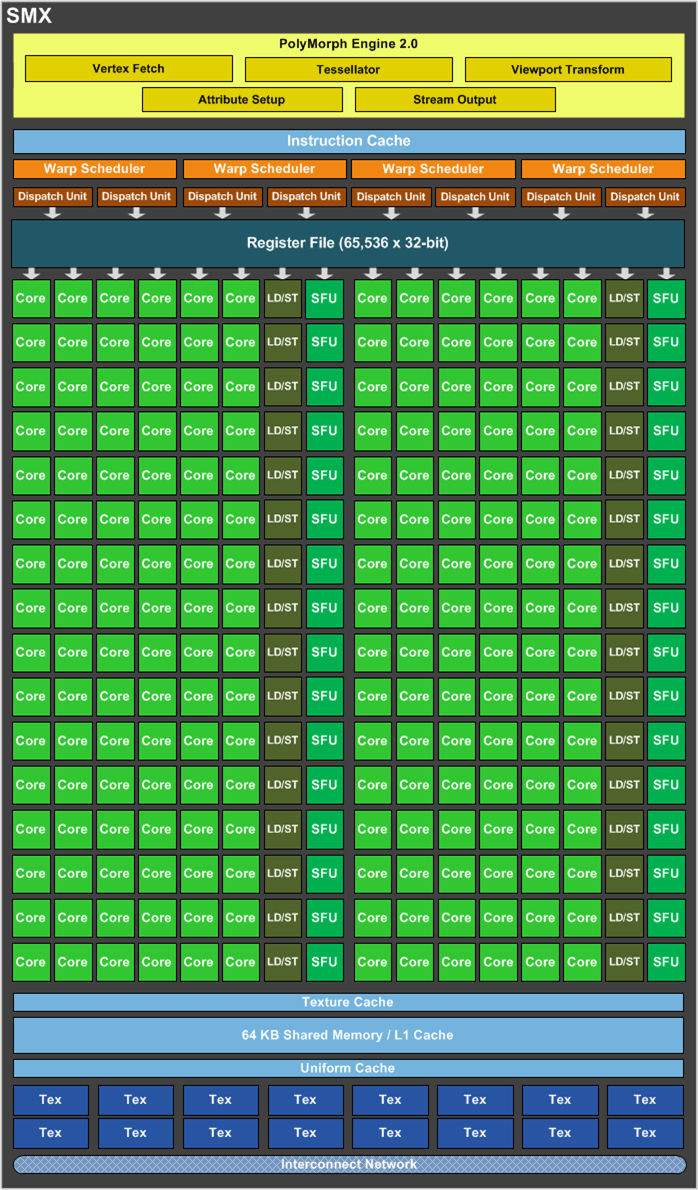
\includegraphics[width=\textwidth]{GPU/GeForceGTX680SMX.png}
\caption{NVIDIA GeForce GTX680 SMX. Source: NVIDIA.}
\label{GPU:GeForceGTX680SMX}
\end{figure}

CUDA is a combination hardware/software platform that enables NVIDIA GPUs to execute programs written in C, C++, Fortran, and other languages. A CUDA program invokes parallel functions called kernels that execute across many parallel threads. The programmer or compiler organizes these threads into thread blocks and grids of thread blocks, as shown in Figure \ref{GPU:CUDAMemoryHierarchy}. Each thread within a thread block executes an instance of the kernel. Each thread also has thread and block IDs within its thread block and grid, a program counter, registers, per-thread private memory, inputs, and output results.

A thread block is a set of concurrently executing threads that can cooperate among themselves through barrier synchronization and shared memory. A thread block has a block ID within its grid. A grid is an array of thread blocks that execute the same kernel, read inputs from global memory, write results to global memory, and synchronize between dependent kernel calls. In the CUDA parallel programming model, each thread has a per-thread private memory space used for register spills, function calls, and C automatic array variables. Each thread block has a per-block shared memory space used for inter-thread communication, data sharing, and result sharing in parallel algorithms. Grids of thread blocks share results in Global Memory space after kernel-wide global synchronization.

CUDA's hierarchy of threads maps to a hierarchy of processors on the GPU; a GPU executes one or more kernel grids; a streaming multiprocessor (SMX) executes one or more thread blocks; and CUDA cores and other execution units in the SMX execute thread instructions. The SMX executes threads in groups of 32 threads called warps. While programmers can generally ignore warp execution for functional correctness and focus on programming individual scalar threads, they can greatly improve performance by having threads in a warp execute the same code path and access memory with nearby addresses.

\begin{figure}
\centering
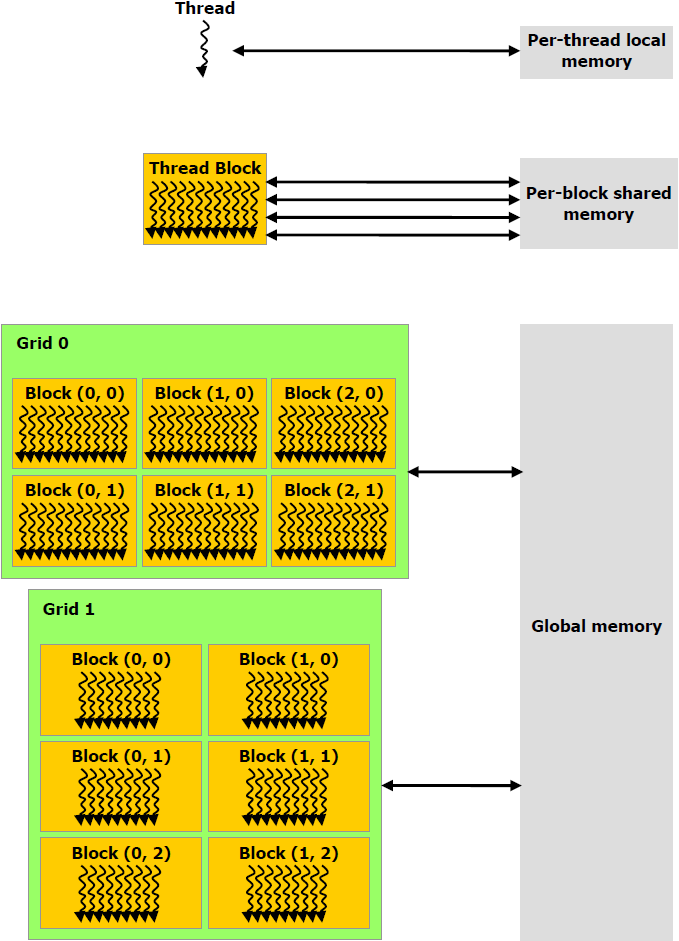
\includegraphics[width=\textwidth]{GPU/CUDAMemoryHierarchy.png}
\caption{CUDA hierarchy of threads, blocks, and grids, with corresponding per-thread private, per-block shared, and per-application global memory spaces. Source: NVIDIA.}
\label{GPU:CUDAMemoryHierarchy}
\end{figure}

\section{Software as a Service}

Ten Simple Rules for Getting Ahead as a Computational Biologist. Make software and website count \citep{260}
% \citep{677}
DOCK BLASTER
wwLigCSRre
ZINCPharmer


\chapterend
